%\documentclass[final]{siamltex}
\documentclass{article}
%\documentclass[final,leqno]{siamltex704}$  $
%\documentclass[final,leqno,onefignum,onetabnum]{siamltex1213}

\usepackage[left=1in,top=1in,right=1in,bottom=1in,dvips,letterpaper]{geometry}
%\usepackage{setspace,url}
%\onehalfspacing
%\doublespacing

\usepackage{graphics,graphicx,epstopdf}
%\usepackage[dvips,bookmarks=true,bookmarksnumbered=true,hypertexnames=false,breaklinks=true,colorlinks]{hyperref}

\usepackage{longtable}
\usepackage[tight]{subfigure}
\usepackage{float}


\usepackage[leqno]{amsmath}
\usepackage{amsxtra, amsfonts,amscd,amssymb,  graphicx,epsf}
%amsthm

%\usepackage[algo2e,linesnumbered, vlined,ruled]{algorithm2e}
\usepackage[algo2e, vlined,ruled]{algorithm2e}

\numberwithin{equation}{section}


%\newtheorem{algorithm}{Algorithm}
%\newtheorem{lemma}{Lemma}
%\newtheorem{theorem}{Theorem}
%\newtheorem{proposition}{Proposition}
%\newtheorem{definition}{definition}

%\usepackage{amsthm}
%\newtheorem{theorem}{Theorem}[section]
%\newtheorem{lemma}[theorem]{Lemma}
%\newtheorem{proposition}[theorem]{Proposition}
%\newtheorem{corollary}[theorem]{Corollary}
%\newtheorem{definition}[theorem]{Definition}

%\newtheorem{remark}[theorem]{Remark}
%\newtheorem{example}[theorem]{Example}
%\newtheorem{assumption}[theorem]{Assumption}
%\newtheorem{condition}[theorem]{Condition}




%% new macros
\newcommand{\st}{\mbox{ s.t.}}
\newcommand{\rk}{\mbox{ rank }}
\newcommand{\tr}{\mathrm{tr}}
\newcommand{\real}{\mathrm{Re}}
\newcommand{\imag}{\mathrm{Im}}
\newcommand{\orth}{ \mathrm{orth} }

\newcommand{\skw}{\mathrm{skew}}
\newcommand{\symm}{\mathrm{symm}}

\newcommand{\R}{\mathbb{R}}
\newcommand{\Rn}{\mathbb{R}^{n \times n}}
\newcommand{\Rnp}{\mathbb{R}^{n \times p}}
\newcommand{\C}{\mathbb{C}}
\newcommand{\Cn}{\mathbb{C}^{n \times n}}
\newcommand{\Cnp}{\mathbb{C}^{n \times p}}

\newcommand{\bx}{\bar x}
\newcommand{\bz}{\bar z}

\newcommand{\Hc}{\mathcal{H}}
\newcommand{\M}{\mathcal{M}}
\newcommand{\Mnp}{\mathcal{M}_n^p}
\newcommand{\SM}{\mathcal{M}_n^p}
\newcommand{\F}{\mathcal{F}}
\newcommand{\T}{\mathcal{T}}
\newcommand{\FB}{\mathbb{F}}

\newcommand{\N}{\mathbb{N}}
\newcommand{\cSM}{\mathrm{conv}(\mathcal{M})}
\newcommand{\cSL}{\mathrm{conv}(\mathcal{L})}
\newcommand{\kHM}{\kappa_{H\mathcal M}}
\newcommand{\kH}{\kappa_{H}}
\newcommand{\kC}{\kappa_C}
\newcommand{\kA}{\kappa_A}
\newcommand{\kT}{\kappa_\tau}
\newcommand{\kg}{\kappa_g}

\newcommand{\SP}{{\mathrm{Sp}^{n-1}}}
\newcommand{\nSP}{{\mathrm{Sp}}}
\newcommand{\pS}{{\mathcal{S}^{n}}}

\newcommand{\HB}{\mathcal{H}}
\newcommand{\BB}{\mathcal{B}}
\newcommand{\UB}{\mathbb{U}}
\newcommand{\VB}{\mathbb{V}}

\newcommand{\Ub}{\mathbf{U}}
\newcommand{\Vb}{\mathbf{V}}
\newcommand{\Wb}{\mathbf{W}}
\newcommand{\Ib}{\mathbf{I}}
\newcommand{\Hb}{\mathbf{H}}
\newcommand{\xb}{\mathbf{x}}
\newcommand{\Dcal}{\nabla}
\newcommand{\nb}{\mathbf{n}}
\newcommand{\drm}{\mathrm{d}}
\newcommand{\br}{\mathbb{R}}


\newcommand{\LCal}{\mathcal{L}}
\newcommand{\sign}{\mathrm{SGN}}
\newcommand{\sgn}{\mathrm{sgn}}
\newcommand{\vzero}{\mathbf{0}}
\newcommand{\vone}{{\mathbf{1}}}
\newcommand{\Prob}{{\mathrm{Prob}}}

\newcommand{\ve}{{\mathrm{vec}}}
\newcommand{\mat}{{\mathrm{mat}}}
\newcommand{\vdiag}{\widetilde\mathrm{Diag}}

\newcommand{\half}{\frac{1}{2}}

%\newcommand{\D}{\mathcal{D}}
\newcommand{\D}{\nabla}
\newcommand{\G}{\mathcal{G}}

\newcommand{\iprod}[2]{\left \langle #1, #2 \right \rangle }
\newcommand{\rprod}[2]{\Re \left \langle #1, #2 \right \rangle }

\newcommand{\shrink}{\mathcal{S}}

\newcommand{\be}{\begin{equation}}
\newcommand{\ee}{\end{equation}}
\newcommand{\bee}{\begin{equation*}}
\newcommand{\eee}{\end{equation*}}
\newcommand{\bea}{\begin{eqnarray}}
\newcommand{\eea}{\end{eqnarray}}
\newcommand{\beaa}{\begin{eqnarray*}}
\newcommand{\eeaa}{\end{eqnarray*}}



%\usepackage[usenames]{color}
\usepackage[normalem]{ulem}
\newcommand{\remove}[1]{{\color{Gray}\sout{#1}}}
\newcommand{\comm}[1]{{\color{red}#1}}
\newcommand{\revise}[1]{{\color{blue}#1}}

\newcommand{\dx}[2]{\frac{d#1}{d #2}}
\newcommand{\dxf}[1]{\frac{d}{d #1}}
\newcommand{\ddx}[2]{\frac{d^2 #1}{d #2 ^2}}
\newcommand{\paruxf}[1]{\frac{\partial }{\partial #1}}
\newcommand{\parux}[2]{\frac{\partial #1}{\partial #2}}

\begin{document}
\title{Mini-project}

\author{ZHU, Weizhi \; HKUST\\
FAN, Min \; HKUST}
\maketitle
%\lecture{Lecture X. Title Here}{Yuan Yao}{Your Name}{Date here}
%\setcounter{section}{0}
\section{Coauthorship detection}
  In this part, we focus on the data of Coauthership matrix as follow:

CA coauthorAdj.txt - 3607x3607 adjacency matrix of the coauthorship network. More preciously, the $(i,j)$-th entry of CA is 1 if authors i and j had coauthored at least one paper, 0 otherwise.

CAG coauthorAdjGiant.txt - 2263x2263 adjacency matrix of the giant component of the coauthorship network where each edge denotes at least t=1 paper coauthored. That is to say, the graph CA has many disjiont subgraphs. And CAG is the giant component subgraph of CA.

We let CAT denote the Threshold adjacency matrix whose $(i,j)$-th entry is 1 if authors i and j had coauthored at least two papers, 0 otherwise.
CATG coauthorAdjThreshGiant.txt -  236x236 adjacency matrix of the giant component of the graph CAT.

ACA authorCiteAdj.txt - 3607x3607 adjacency matrix whose $(i,j)$-th entry is 1 if author i cites author j at least once, 0 otherwise. And ACAG authorCitAdjGiant.txt - 2654x2654 adjacency matrix is a giant component of graph of ACA.

We will firstly detect the connect component of original coauthorship adjancency matrix CA by \textbf{Fiedler Theroy}, the disconnection distinguishes in most apparent way: people in each connect component do not cooperate.

Then we further dectect community in the largest connect component, with adjacency matrix CATG(or CAG), lots of clustering method could be applied here, such as \textbf{Minimizing Cut},\textbf{Minimizing distance/probability of transition in different clusters},\textbf{SCORE method} and so on. We try to give some explantion in different community dection and compare each result.


\subsection{Connect component dectection}
\subsection{Community dectection}
As we have introduced at the begin of this section, we will do community dectection of the largest connenct component CATG. The first method we apply is to \textbf{minimize} cut, for a given k,
\begin{equation}
\begin{aligned}
& RatioCut(A_1,...,k) = \sum_{i=1}^k \frac{cut(A_i,A_i^c)}{|A_i|}\\
& Ncut(A_1,...,A_k) = \sum_{i=1}^k \frac{cut(A_i,A_i^c)}{Vol(A_i)}\\
\end{aligned}
\end{equation}
However, the combination optimization is NP-hard, we using \textbf{Spectral Method} as a relaxation to dectect the community, such as \textbf{Normalized Laplacian}, \textbf{Unnormalized Laplacian} and \textbf{Cheeger bipartition}.

Before we introduce several algorithms, we firstly give a breif introduction on graph Laplacian. Given an adjacent matrix $A^{n\times n}$, firstly we consider the case of undirected graph, i.e.$a_{ij} = a_{ji}$:

Let $D = diag(d_i), d_i = \sum_{j=1}^n A_{ij}$, then unnormalized Laplacian is defined as $L = D - A$, normalized Laplacian is defined as $\mathcal{L} = D^{-1/2}LD^{-1/2}$, and the probability transition matrix is defined as $P = D^{-1}L$.

Algorithm of Unnormalized Laplacian Spectral Clustering is given below,

\begin{algorithm2e}[H]\caption{Unnormalized spectral clustering}
	\textbf{Input} Similarity matrix $S\in \textrm{R}^{n\times n}$, number $k$ of clusters to construct
	initial $r_0 = b$ , $x_0=0$ , $S_0=\emptyset$\\
	 Construct
	 a similarity graph by one of the ways described in Section 2. Let $W$ be its weighted adjacency matrix.\\
	Compute the unnormalized Laplacian $L$.\\
	Compute the first $k$ eigenvectors $v_1 ,\cdots,v_k$ of $L$.\\
	Let $V \in \textrm{R}^{n\times k}$ be the matrix containing the vectors $v_1 ,\cdots,v_k$ as columns. \\
	For $i = 1,\cdots,n$, let $y_i\in \textrm{R}^k$ be the vector corresponding to the $i$-th row of $V$.\\
    Cluster the points $(y_i)_{i=1,\cdots,n}$ in $\textrm{R}^{k}$ with the $k$-means algorithm into clusters $C_1 ,\cdots,C_k$.\\
	\textbf{Output} Clusters $A_1 ,\cdots,A_k$ with $A_i = \{j| y_j \in C_i \}$.
\end{algorithm2e}

The unnormalized one is basically similar which we omit. Cheeger's bipartition will be done in the final project.

Now, we turn to SCORE, that is, Spectral Clustering On Ratios of Eigenvectors.SCORE is a recent spectral method proposed by Jin [24]. This method tends to be reasonable because the ratios of eigenvectors are proportion to the heterogeneity parameters. Assume $K$ (number of communities) as known and let $A$ be the adjacency matrix associated with $\mathcal{N}$:
	\[
	A(i,j)=\left\{
	\begin{array}{ll}
	1, & \hbox{if there is an edge between node $i$ and $j$,} \\
	0, & \hbox{otherwise;}
	\end{array}
	\right.
	\]
	note that $A$ is symmetric. SCORE consists of the following simple steps.
	\begin{itemize}
		\item Let $\hat{\xi}_1,\hat{\xi}_2,\cdots,\hat{\xi}_K$ be the first $K$ (unit-norm) eigenvectors of $A$. Obtain the $n \times (K-1)$ matrix $\hat{R}$ by $\hat{R}(i,k)=\hat{\xi}_{k+1}(i)/\hat{\xi}_1(i),1 \leq i \leq n,1\leq k\leq K-1$.
		\item Clustering by applying the classical k-means to $\hat{R}$, assuming there are $\leq K$ communities.
	\end{itemize}
Besides NSC,BCPL,APL method will be tried in final project.

Now we give the experiment result:

\begin{figure}[H]
	\centering
	% 	 Requires \usepackage{graphicx
	\includegraphics[width=0.7\textwidth]{compare-2/giantcoau-score-2.png}
	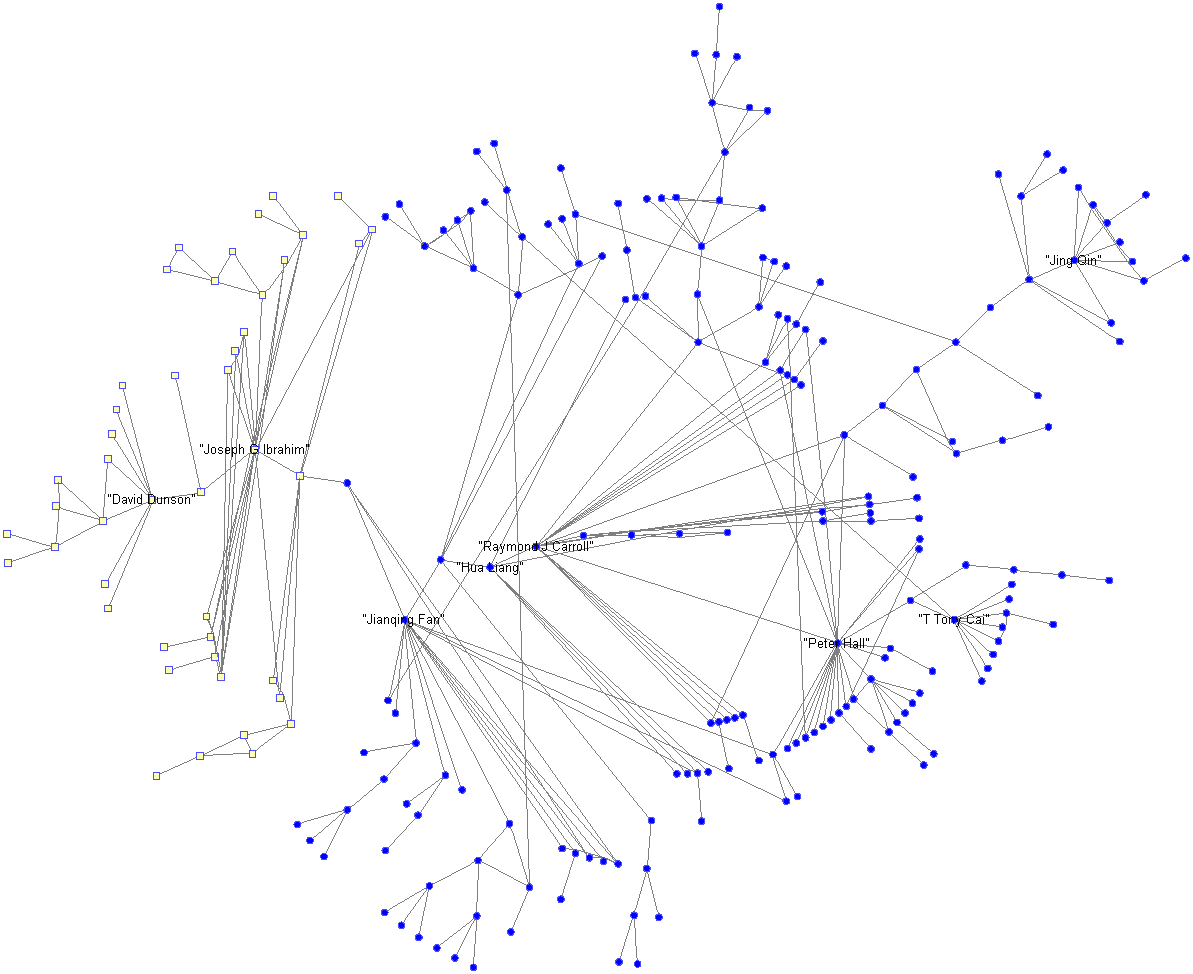
\includegraphics[width=0.7\textwidth]{compare-2/giantcoau-spcunl-2.png}
	\caption{Setting the cluster numbers $K=2$. Comparing Spectral method (top) and SCORE method (bottom), different color implies different clusters. Note that different Spectral method coincide when $K=2$. }
\end{figure}

Firstly, we set the cluster number to be $K=2$ (Figure 1), in this case, three different spectral methods give exactly same clusterings. But SCORE method performs a little different at the edge of two clusterings. More explanation may be further explored in final project.

\begin{figure}[H]
	\centering
	% 	 Requires \usepackage{graphicx
	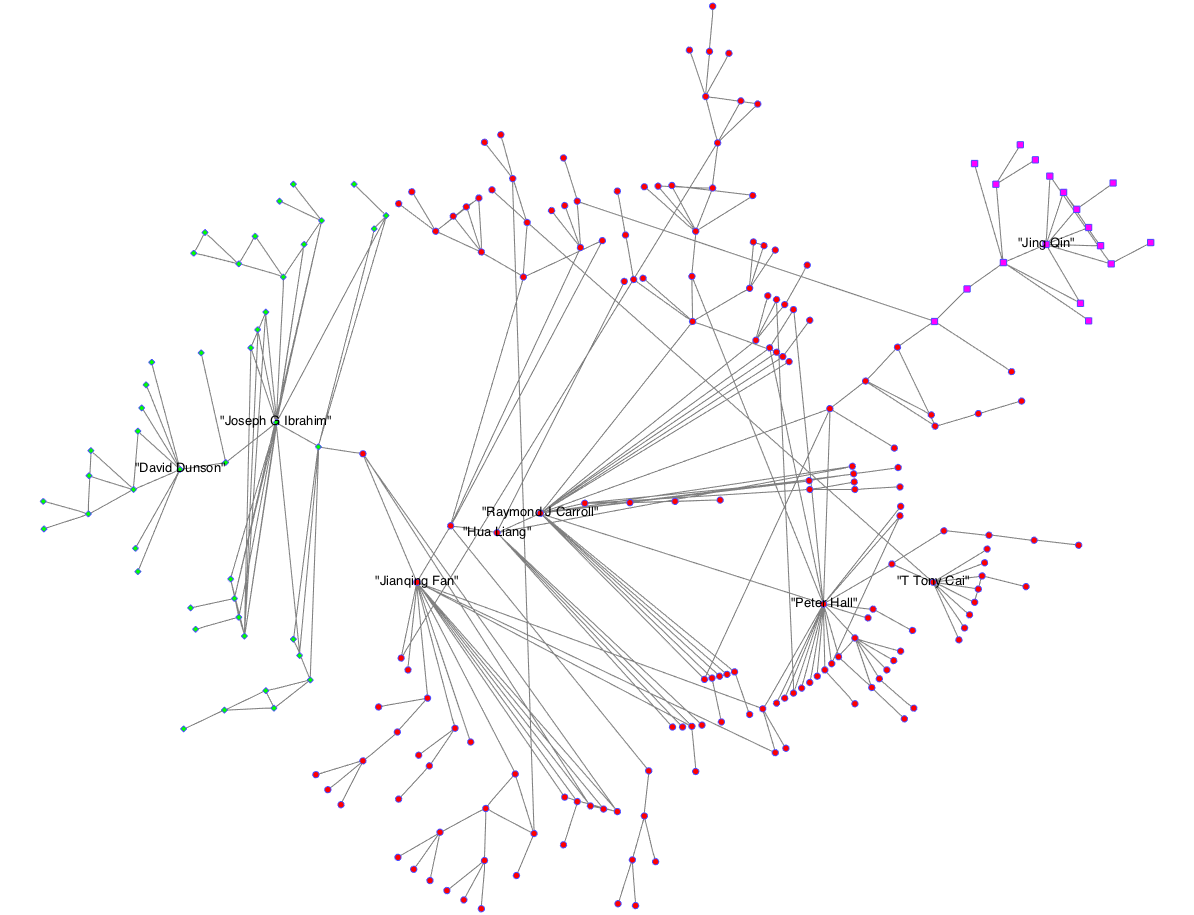
\includegraphics[width=0.7\textwidth]{compare-3/giantcoau-spcnsym-3.png}
	\includegraphics[width=0.7\textwidth]{compare-3/giantcoau-score-3.png}
	\caption{Setting the cluster numbers $K=3$. Comparing Spectral method with Normalized Laplacian (top) and SCORE method (bottom), different color implies different clusters.Authors with more than 8 cooperators has been named in the figure}
\end{figure}

Then, the case of $K=3$. Different methods present different incline for clustering, not only different in the edge. For example (Figure 2), spectral method(Normalized Laplacian) detect "Divid Dunson", "Jianqing Fan" and  "Jing Qin" communities, as we explain for intuitive meaning of cutting, we may regard this three communities do not intend to cooperate with others. However, SCORE method further bipartition "Divid Dunson" community instead of dectect "Jing Qin" community, which means SCORE method are inclined to regard "Jing Qin" and "Jianqing Fan" as one.

We can introduce Adjuested Rand Index (ARI) and Variation Information (VI) to measure the similarity of different clusterings. ARI and VI are given as follow:
	\[ \begin{aligned}
	& ARI=\frac{\sum_{ij}\binom{n_{ij}}{2}-\left[\sum_i\binom{a_i}{2}\sum_{j}\binom{b_j}{2}\right]/ \binom{n}{2}}{\frac{1}{2}\left[\sum_i\binom{a_i}{2}+\sum_{j}\binom{b_j}{2}\right]-\left[\sum_i\binom{a_i}{2}\sum_{j}\binom{b_j}{2}\right]/ \binom{n}{2}} \\
	& VI(X;Y)=-\sum\limits_{i,j} r_{ij}[\log(r_{ij}/p_i)+\log(r_{ij}/q_j)]
	\end{aligned}\]
Lager ARI and less VI will ensure the consistency of the two partitions.

\begin{table}\caption{K = 2}
	\centering
	\begin{tabular}{|c|c|c|c|c|}
		% after \\: \hline or \cline{col1-col2} \cline{col3-col4} ...
		\hline
		& SCORE & SpCUL & SpCNL-sym & SpCNL-rw \\\hline
		SCORE & 1.00/0.00 & 0.8399/27.3041 & 0.8399/27.3041 & 0.8399/27.3041 \\\hline
		SpCUL &  & 1.00/0.00 & 1.00/0.00 & 1.00/0.00 \\\hline
		SpCNL-sym &  &  & 1.00/0.00  & 1.00/0.00 \\\hline
		SpCNL-rw &  &  &  & 1.00/0.00 \\\hline
	\end{tabular}
\end{table}

\begin{table}\caption{K =3}
	\centering
	\begin{tabular}{|c|c|c|c|c|}
		% after \\: \hline or \cline{col1-col2} \cline{col3-col4} ...
		\hline
		& SCORE & SpCUL & SpCNL-sym & SpCNL-rw \\\hline
		SCORE & 1.00/0.00 & 0.6023/45.4977 & 0.5924/46.2624 & -0.0901/64.5352 \\\hline
		SpCUL &  & 1.00/0.00 & 0.9859/3.3394 & 0.3517/40.9162 \\\hline
		SpCNL-sym &  &  & 1.00/0.00  & 0.3422/44.2556 \\\hline
		SpCNL-rw &  &  &  & 1.00/0.00 \\\hline
	\end{tabular}
\end{table}

\begin{figure}[H]
	\centering
	% 	 Requires \usepackage{graphicx
	\includegraphics[width=0.7\textwidth]{trend/giantcoau-score-2.png}
	\includegraphics[width=0.7\textwidth]{trend/giantcoau-score-3.png}
	\caption{Focusing on SCORE method, $k=2$ (top) and $k=3$ (bottom) are shown.}
\end{figure}

\begin{figure}[H]
	\centering
	% 	 Requires \usepackage{graphicx
	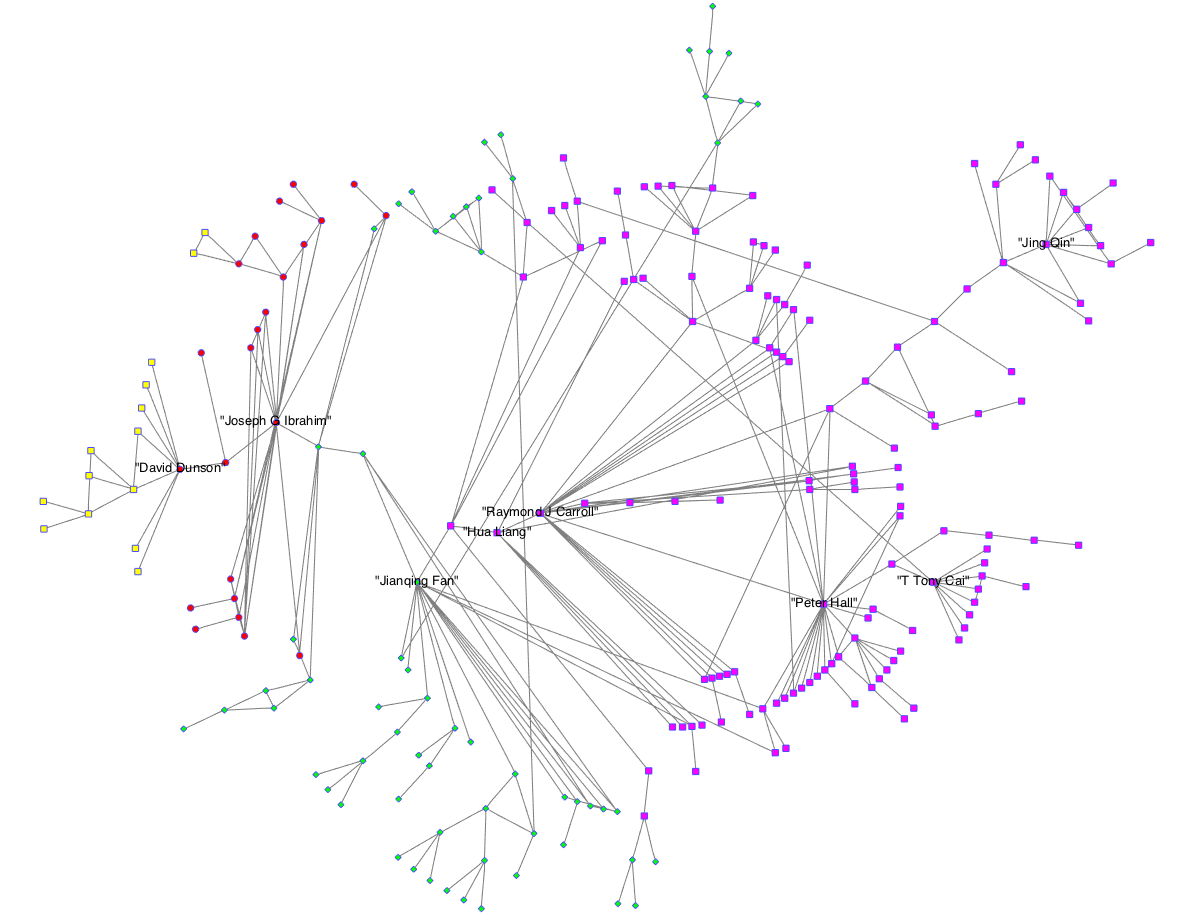
\includegraphics[width=0.7\textwidth]{trend/giantcoau-score-4.png}
	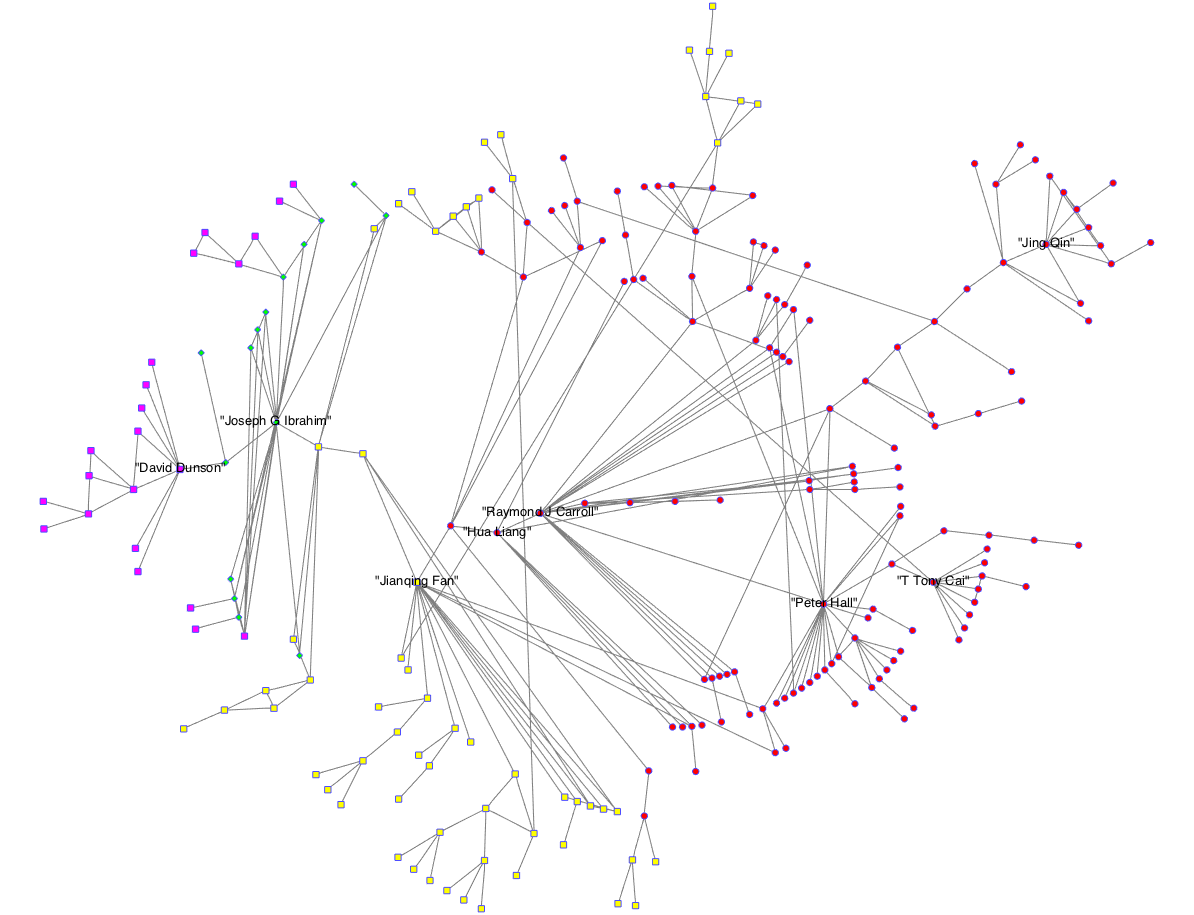
\includegraphics[width=0.7\textwidth]{trend/giantcoau-score-5.png}
	\caption{Focusing on SCORE method, $k=4$ (top) and $k=5$ (bottom) are shown.}
\end{figure}

Finally, we focus the SCORE Method to see the trand as $k$ increase(Figure 3 and Figure 4). In fact, more clusterings are dectected, continue to $k=3$, "Jianqing Fan" community is been furthered partitioned.

\section{Citation community detection}
Now we focus on the citation network CAG which is a directed graph. A efficient method for the communities detection will be introduced briefly below.
Direct SCORE (D-SCORE) is commuity detection method which constructs two associated undirected graphs and then uses SCORE method to do the futher community clustering. For detailed explanations, see the forthcoming manuscript [23]. Given a directed network $\mathcal{N} = (V,E)$, assume $\mathcal{N}$ has $K$ communities. Let $A$ be the adjacency matrix, and let $\hat{u}_1,\hat{u}_2,\cdots,\hat{u}_K$ and $\hat{v}_1,\hat{v}_2,\cdots,\hat{v}-K$ be the first $K$ left singular vectors and the first $K$ right singular vectors of $A$, respectively. Also, define two associated (undirected) networks with the same set of nodes as follows
	\begin{itemize}
		\item \emph{Citer network.} There is an (undirected) edge between two distinct nodes $i$ and $j$ in $V$ if and only if both of them have cited a node $k$ at least once, for some $k \in (V \backslash \{i,j\})$ (i.e., they have a common citee).
		\item \emph{Citee network.} There is an (undirected) edge between two distinct node $i$ and $j$ in $V$ if and only if each of them has been cited at least once by the same node $k \notin (V \backslash \{i,j\})$ (i.e., they have a common citer).
	\end{itemize}
	
	
	\def\sgn{\mathop{\rm sgn}}
	
	Let $\mathcal{N}_1$ and $\mathcal{N}_2$ be the giant components of the Citer network and Citee network, respectively. Define two $n \times (K-1)$ matrices $\hat{R}^{(l)}$$\hat{R}^{(r)}$ by
	\[
	\hat{R}^{(l)}(i,k)=\left\{
	\begin{array}{ll}
	\sgn (\hat{u}_{k+1}(i)/\hat{u}_1(i))\cdot \min\{|\frac{\hat{u}_{k+1}(i)}{\hat{u}_{1}(i)}|,\log (n)\}, & \hbox{$i \in \mathcal{N}_1$}\\
	0, & \hbox{$i \notin \mathcal{N}_1$}.
	\end{array}
	\right.
	\]\[
	\hat{R}^{(r)}(i,k)=\left\{
	\begin{array}{ll}
	\sgn (\hat{v}_{k+1}(i)/\hat{v}_1(i))\cdot \min\{|\frac{\hat{v}_{k+1}(i)}{\hat{v}_{1}(i)}|,\log (n)\}, & \hbox{$i \in \mathcal{N}_2$} \\
	0, & \hbox{$i \notin \mathcal{N}_2$}.
	\end{array}
	\right.
	\]
	Note that all nodes split into four disjoint subsets:
	\[
	\mathcal{N} = (\mathcal{N}_1 \cap \mathcal{N}_2 ) \cup (\mathcal{N}_1 \backslash \mathcal{N}_2 ) \cup (\mathcal{N}_2 \backslash \mathcal{N}_1 ) \cup (\mathcal{N} \backslash (\mathcal{N}_1 \cup \mathcal{N}_2 )).
	\]
	
	D-SCORE clusters nodes in each subset separately.
	\begin{enumerate}
		\item $(\mathcal{N}_2 \cap \mathcal{N}_1).$ Restricting the rows of $\hat{R}^{(l)}$ and $\hat{R}^{(r)}$ to the set $\mathcal{N}_2 \cap \mathcal{N}_1$ and obtaining two matrices $\tilde{R}^{(l)}$ and $\tilde{R}^{(r)}$, we cluster all nodes in $\mathcal{N}_2 \cap \mathcal{N}_1$ by applying the $k$-means to the matrix $[\tilde{R}^{(l)},\tilde{R}^{(r)}]$ assuming there are $\leq K$ communities.
		\item $(\mathcal{N}_2 \backslash \mathcal{N}_1)$.  Note that according to the communities we identified above,
		the rows of $\tilde{R}^{(l)}$ partition into $\leq K$ groups. For each group, we call the mean of the row vectors the \emph{community center}. For a node i in $\mathcal{N}_2 \backslash \mathcal{N}_1$, if the $i$-th row of  $\hat{R}^{(l)}$ is closest to the center of the $k$-th community for some $1 \leq k \leq K$, then we assign it to this community.
		\item  $(\mathcal{N}_2 \backslash \mathcal{N}_1)$. We cluster in a similar fashion to that in the last step, but we use $(\tilde{R}^{(r)},\hat{R}^{(r)})$ instead of $(\tilde{R}^{(l)},\hat{R}^{(l)})$.
		\item  $(\mathcal{N} \backslash (\mathcal{N}_1\cup \mathcal{N}_2))$.  We say there is a weak-edge between $i$ and $j$ if there
		is an edge between $i$ and $j$ in the weakly connected citation network. By 1-2, all nodes in $\mathcal{N}_1\cup \mathcal{N}_2$ partition into $\leq K$ communities. For each node in $\mathcal{N} \backslash (\mathcal{N}_1\cup \mathcal{N}_2)$, we assign it to the community to which it has the largest number of weak-edges.
	\end{enumerate}
\begin{figure}[H] \label{fig:kmeans}
	\centering
	% 	 Requires \usepackage{graphicx
	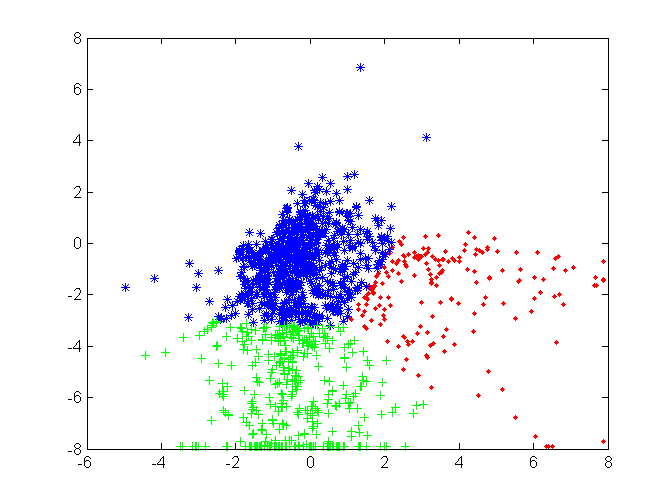
\includegraphics[width=0.4\textwidth]{Dscore/cite-dscore-3-l.png}
	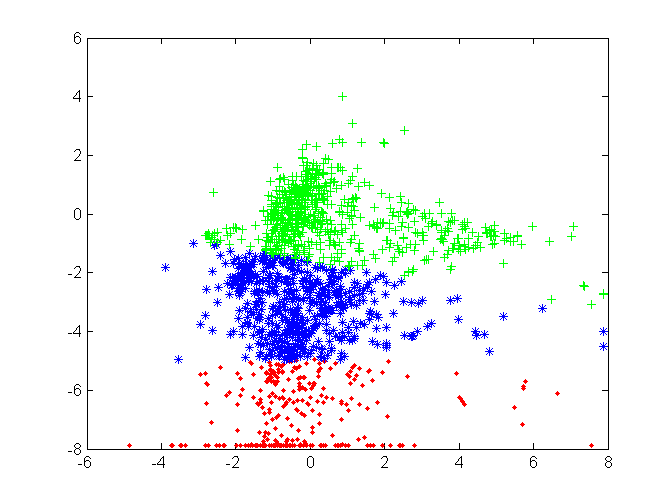
\includegraphics[width=0.4\textwidth]{Dscore/cite-dscore-3-r.png}
	\caption{Left, do clustering by the left singular vector ratios; Right, do clustering by the left singular vector ratios.}
\end{figure}
From Figure 5, we see the communities detected by left and right singular vector ratios have no significant difference. This also confirms the D-SCORE method is reasonable.
 
\begin{figure}[H] \label{fig:kmeans}
	\centering
	% 	 Requires \usepackage{graphicx
	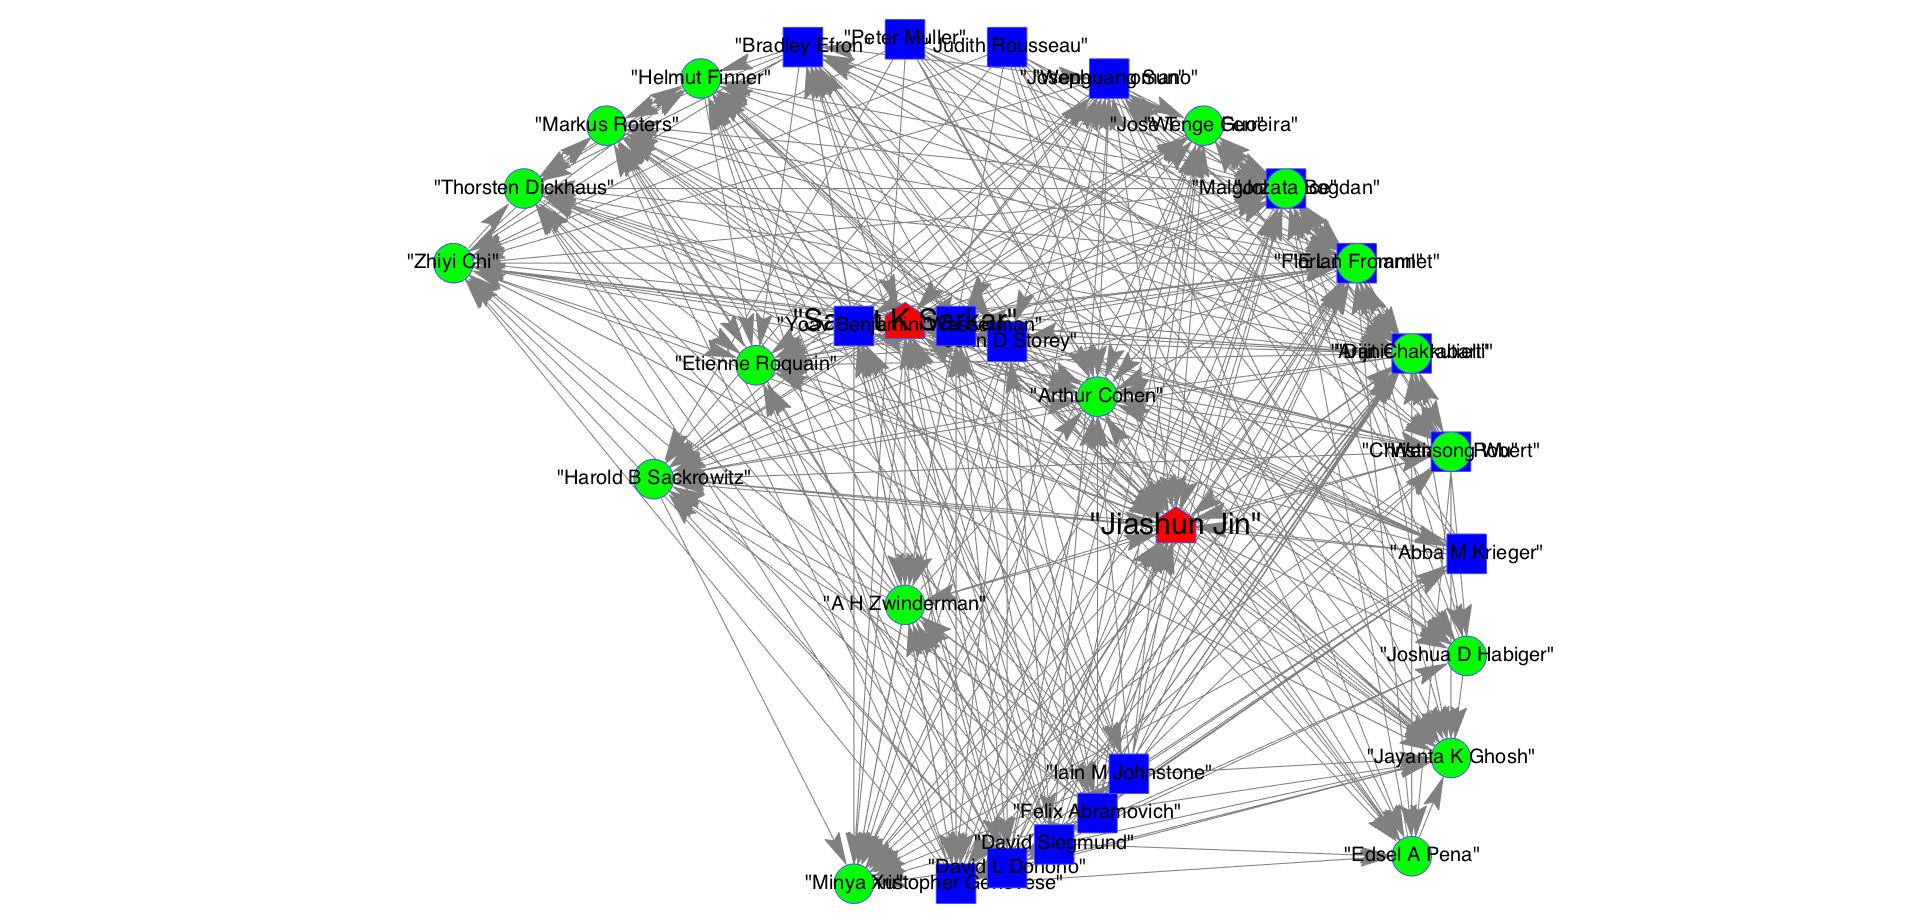
\includegraphics[width=\textwidth]{Dscore/dsocre-1-ah.png}
	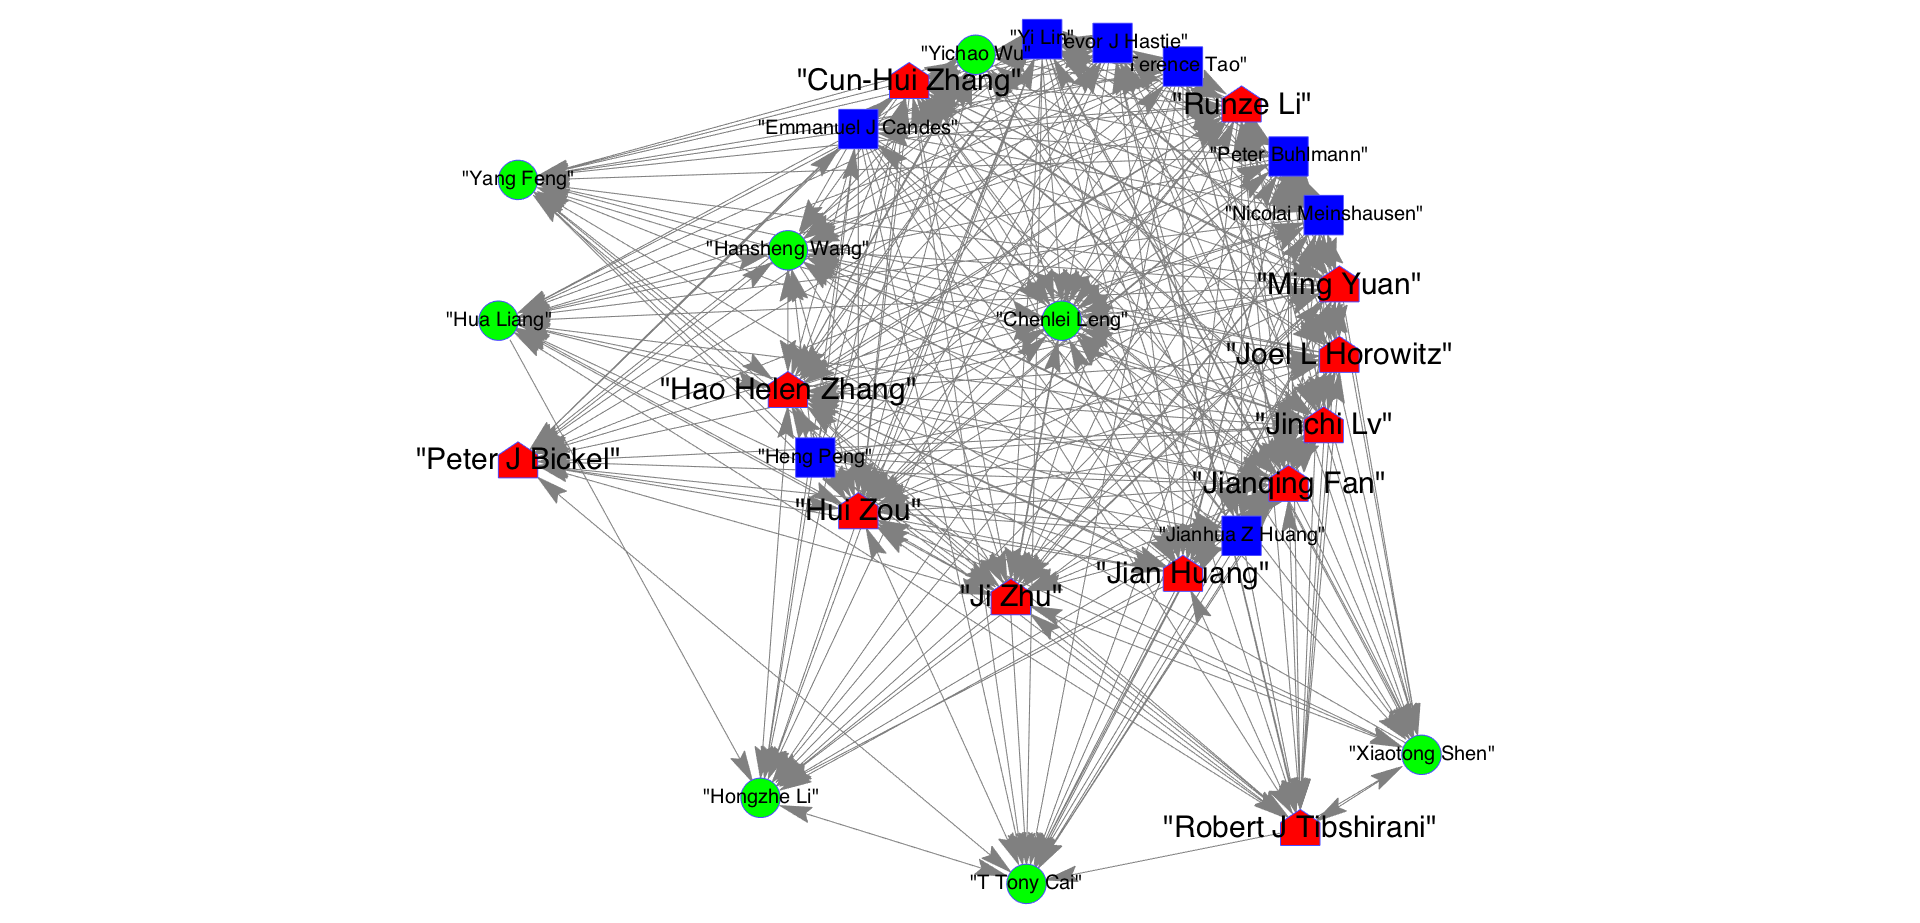
\includegraphics[width=\textwidth]{Dscore/dsocre-2-ah.png}
	\caption{K = 3, Communities with 1285 nodes, 359 nodes and 1010 nodes respectively. Top, community with 1285 nodes, only nodes with most 10 authority and hub are shown; Bottom, community with 1285 nodes, only nodes with most 10 authority and hub are shown.}
\end{figure}

\textbf{1-community}
top20aut: "Jianqing Fan", "Chenlei Leng", "Ji Zhu", "Hui Zou", "Hua Liang", "Runze Li", "T Tony Cai", "Hansheng Wang", "Cun-Hui Zhang", "Hongzhe Li", "Ming Yuan", "Hao Helen Zhang", "Robert J Tibshirani", "Yang Feng", "Jian Huang", "Joel L Horowitz", "Jinchi Lv", "Xiaotong Shen", "Yichao Wu", "Peter J Bickel".

top20hub:"Jianqing Fan", "Hui Zou", "Peter Buhlmann", "Nicolai Meinshausen", "Yi Lin", "Ming Yuan", "Trevor J Hastie", "Runze Li", "Emmanuel J Candes", "Cun-Hui Zhang", "Heng Peng", "Jian Huang", "Peter J Bickel", "Terence Tao", "Jinchi Lv", "Robert J Tibshirani", "Ji Zhu", "Hao Helen Zhang", "Joel L Horowitz", "Jianhua Z Huang".

\textbf{2-community}

top20aut: "Jayanta K Ghosh", "Arijit Chakrabarti", "Florian Frommlet", "Malgorzata Bogdan", "Jiashun Jin", "Etienne Roquain", "Sanat K Sarkar", "Thorsten Dickhaus", "Helmut Finner", "Markus Roters", "Zhiyi Chi"
"Minya Xu", "Harold B Sackrowitz", "Arthur Cohen", "Wensong Wu", "Joshua D Habiger", "Edsel A Pena", "Wenge Guo", "A H Zwinderman", "Jose T A S Ferreira".

top20hub: "John D Storey", "Larry Wasserman", "Christopher Genovese", "Yoav Benjamini", "David Siegmund", "David L Donoho", "Bradley Efron", "Iain M Johnstone", "Jiashun Jin", "Sanat K Sarkar", "Daniel Yekutieli"
"Felix Abramovich", "Abba M Krieger", "Joseph P Romano", "E L Lehmann", "John Rice", "Wenguang Sun", "Christian P Robert", "Judith Rousseau", "Peter Muller".

As we’ve shown in Figure 8, three communities are detected, we do some remarks as follow:
\begin{enumerate}
\item Almost all Top-20-aut and Top-20-hub are in the same community, community with 359 nodes. We conclude this community as a “Self-Loop” community. They merely cite researcher out of this community for their Authority in this area.
\item As [2] suggests, three communities detected here could regarded as “Large-Scale Multiple Testing” ,“Variable Selection” and “Spatial and Semi-parametric/Nonparametric Statistics” communities.
\item Citation community detection base on citee and citer, while coauthorship community detection base on operation, they differs a lot.
\end{enumerate}

\bibliographystyle{plain}
%\bibliography{TBA-bib}
\begin{thebibliography}{99}

\bibitem{BAnon} {\sc Bickel, P. J., and A. Chen}, {\em A nonparametric view of network models and Newman-Girvan and other modularities}, Proceedings of the National Academy of Sciences of the United States of America 106.50(2009):21068-73.

\bibitem{Jfast}
{\sc Jin, Jiashun}, {\em Fast community detection by SCORE}, Annals of Statistics 43.2(2012):672-674.

\bibitem{JJcoau}
{ \sc Ji, Pengsheng, and J. Jin}, {\em Coauthorship and Citation Networks for Statisticians}, Eprint Arxiv (2014).

\end{thebibliography}

\end{document}


